\section{Topic}
\label{sec:topic}



\subsection{Constraint Graph}
\begin{figure}[htb]
    \begin{center}
        \begin{tabular}{cc}
            \begin{minipage}{0.45\linewidth}
                \begin{center}
                    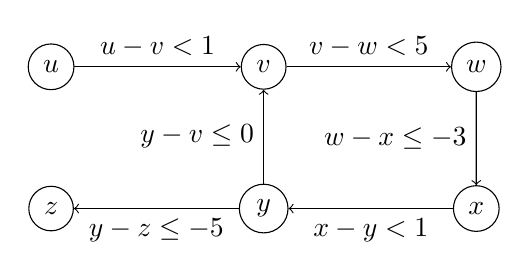
\begin{tikzpicture}[scale=0.9,state/.style={draw, circle, fill=none,text centered, text=black}]
    \node[state] (u) at (0, 2) {$u$};
    \node[state] (v) at (3, 2) {$v$};
    \node[state] (w) at (6, 2) {$w$};
    \node[state] (x) at (6, 0) {$x$};
    \node[state] (y) at (3, 0) {$y$};
    \node[state] (z) at (0, 0) {$z$};
    \draw [->] (u) -- node[anchor=south] {$ u-v < 1 $} (v);
    \draw [->] (v) -- node[anchor=south] {$ v-w < 5 $} (w);
    \draw [->] (w) -- node[anchor=east] {$ w-x \leq -3 $} (x);
    \draw [->] (x) -- node[anchor=north] {$ x-y < 1 $} (y);
    \draw [->] (y) -- node[anchor=north] {$ y-z \leq -5 $} (z);
    \draw [->] (y) -- node[anchor=east] {$ y-v \leq 0 $} (v);
\end{tikzpicture}

                \end{center}
            \end{minipage}
            &
            \begin{minipage}{0.45\linewidth}
                \begin{center}
                    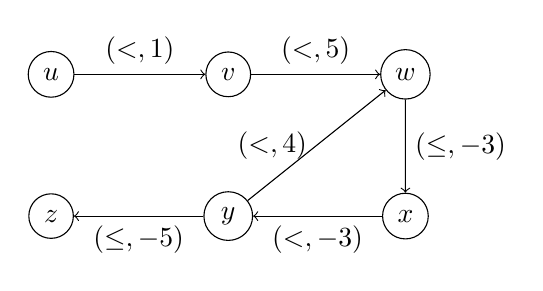
\begin{tikzpicture}[scale=0.9,state/.style={draw, circle, fill=none,text centered, text=black}]
    \node[state] (u) at (0, 2) {$u$};
    \node[state] (v) at (2.5, 2) {$v$};
    \node[state] (w) at (5, 2) {$w$};
    \node[state] (x) at (5, 0) {$x$};
    \node[state] (y) at (2.5, 0) {$y$};
    \node[state] (z) at (0, 0) {$z$};
    \draw [->] (u) -- node[anchor=south] {$ (<,1) $} (v);
    \draw [->] (v) -- node[anchor=south] {$ (<,5) $} (w);
    \draw [->] (w) -- node[anchor=west] {$ (\leq,-3) $} (x);
    \draw [->] (x) -- node[anchor=north] {$ (<,-3) $} (y);
    \draw [->] (y) -- node[anchor=north] {$ (\leq,-5) $} (z);
    \draw [->] (y) -- node[anchor=east] {$ (<,4) $} (w);
\end{tikzpicture}

                \end{center}
            \end{minipage}
        \end{tabular}
    \end{center}
    \caption{Examples of constraint graphs for
        Equation~\ref{eq:example-2} (left) and
        Equation~\ref{eq:example-3} (right).}
    \label{fig:contraints-graphs}
\end{figure}
Constraint graph (Figure~\ref{fig:contraints-graphs})
is a weighted directed graph which is used by the DL
constraints checker
(Figure~\ref{fig:lazy-and-incremental-approaches}) to check
if the given DL constraints are satisfiable.
Let $ \phi $ be a conjunction of DL constraints (\ie a DL formula),
let $ \prec \; = \{ <, \leq \} $ be an operation in a DL constraint
$ x - y \prec c \in \phi $ and let variables and constants
in the constraints be defined over a domain $ \mathbb{D} $
(\ie $ x,y,c \in \mathbb{D} $ ) which can be \eg Reals ($ \mathbb{R} $).
Then according to~\cite{cotton2004some} the constraint graph
can be defined as follows:
\begin{definition}[Constraint Graph]
    \label{def:constraint-graph}
    The constraint graph $ \Gamma $ represents a conjunction of
    DL constraints $ \phi $.
    It is a graph $ \Gamma = (V,E,weight,op) $ where:
    \begin{itemize}
        \item $ V $ is a set of vertices. Each vertex $ x \in V $
        corresponds to one numeric variable occurring in some DL constraint
        $ x - y \prec c \in \phi $.
        \item $ E $ is a set of directed edges. Each edge
        $ (x,y) \in E $ corresponds to a DL inequality
        $ x - y \prec c \in \phi $.
        \item $ weight: E \mapsto \mathbb{D} $ is a weight function.
        It maps each edge $ (x,y) \in E $ to the constant
        $ c \in \mathbb{D} $ from the corresponding DL inequality
        $ x - y \prec c \in \phi $.
        \item $ op: E \mapsto \{ <, \leq \} $ is a function which
        maps each edge $ (x,y) \in E $ to the operation
        $ \prec $ from the corresponding DL inequality
        $ x - y \prec c \in \phi $.
    \end{itemize}
\end{definition}




\subsection{Negative Cycles in Constraint Graph}
If a constraint graph has a negative cycle then the corresponding
conjunction of DL constraints $ \phi $ represented by the graph is
not SAT.

A path in the graph corresponds to a sum of the corresponding
constraints. \Eg the path
$ u \rightarrow v \rightarrow w \rightarrow x $
in the left graph on Figure~\ref{fig:contraints-graphs}
corresponds to the following sum of the DL inequalities:
\begin{equation}
    \begin{aligned}
        u - v & < 1 \\
        v - w & < 5 \\
        w - x & \leq -3 \\
        \hline
        u - x & < 3
    \end{aligned}
\end{equation}
If at least one strict inequality is present
then the resulting inequality will also be strict.
This summation along a path can also be expressed with
a transitivity constraint (\eg~Equation~\ref{eq:transitivity-example}).
The transitivity constraint naturally follows from $ \phi $ and
therefore must be satisfied in order to satisfy $ \phi $.

A cycle in the constraint graph corresponds to an inequality
$ 0 \prec c $
which may cause a conflict in the following situations:
\begin{itemize}
    \item $ c < 0$
    \item $ c = 0 $ and $ \prec $ is $ < $
    (can be checked with $ op $ from Definition~\ref{def:constraint-graph})
\end{itemize}

An example of a conflict can be seen on the right graph
on Figure~\ref{fig:contraints-graphs}.
The conflict corresponds to the negative cycle
$ x \rightarrow y \rightarrow w \rightarrow x $
which corresponds to the following inequalities:
\begin{equation}
    \begin{aligned}
        x - y & < -3 \\
        y - w & < 4 \\
        w - x & \leq -3 \\
        \hline
        0 & < -2
    \end{aligned}
\end{equation}



\subsection{Bellman-Ford Algorithm for Constraint Graph}
In~\cite{cotton2004some} a Goldberg-Radzik~\cite{goldberg1993heuristic}
variant of the Bellman-Ford algorithm
(Algorithm~\ref{alg:goldberg-radzik}) is applied to
a constraint graph in order to detect negative cycles.
Important terminology and notation used in the algorithm are given below:
\begin{itemize}
    \item $ d(v) \in \mathbb{D} $ is a distance estimate
    from the source vertex to the given vertex $ v \in V $.
    \item $ \pi(v) \in V $ is a parent of $ v \in V $ in a tree
    of shortest paths. The tree has the source vertex as its root.
    \item $ status(v) = \{ unreached, labelled, scanned \} $ denotes
    if $ v \in V $ has or has not been reached yet or has been marked
    as a scanned \ie processed vertex.
    \item $ r_d(x,y) = weight(x,y) + d(x) - d(y) $ is
    a reduction in distance estimate associated with taking a path
    from the source vertex to $ y \in V $ through $ x \in V $.
    \item Edge $ (x,y) \in E $ is called admissible if $ r_d(x,y) < 0 $
    \ie this edge can improve the current distance estimate for
    the vertex $ y \in V $.
    \item Admissible graph $ \Gamma_d $ is a subgraph
    of $ \Gamma $ composed out of the admissible edges of $ \Gamma $.
\end{itemize}
\begin{Algorithm}
    \caption{Bellman-Ford algorithm takes a graph and a source vertex
        and calculates distances to all other reachable vertices.
        Goldberg-Radzik heuristic, applied to this algorithm,
        suggests to scan a graph in a topological order.}
    \label{alg:goldberg-radzik}
    \begin{algorithm}{Goldberg-Radzik}
        {\text{constraint graph} (V,E,weight,op),
            \text{source vertex} s \in V}
        \CALL{Initialize-Single-Source}((V,E,weight,op), s) \\
        newlyLabelledVertices \= \CALL{Scan}(s) \\
        \begin{WHILE}{newlyLabelledVertices \; is \; not \; empty}
            nextNewlyLabelledVertices \= \varnothing \\
            \begin{FOR}{\mathrm{each \; vertex} \; v \; in \; newlyLabelledVertices}
                t \= \CALL{Scan}(v) \\
                nextNewlyLabelledVertices \= nextNewlyLabelledVertices \cup t
            \end{FOR} \\
            newlyLabelledVertices \= nextNewlyLabelledVertices
        \end{WHILE} \\
        \RETURN False
    \end{algorithm}
\end{Algorithm}

\begin{Algorithm}
    \caption{This procedure initializes distances, parent pointers \etc.}
    \label{alg:init-single-source}
    \begin{algorithm}{Initialize-Single-Source}
        {\text{constraints graph} (V,E,weight,op), \text{source vertex} s}
        \begin{FOR}{\mathrm{each \; vertex} \; v \in V}
            d(v) = \infty \\
            \pi(v) = \NIL \\
            status(v) = unreached
        \end{FOR} \\
        d(s) = 0 \\
        status(s) = labelled
    \end{algorithm}
\end{Algorithm}

\begin{Algorithm}
    \caption{Given a labelled vertex $ v \in V $,
        this procedure tries to improve the distance estimates by
        scanning all the edges outgoing from $ v $.}
    \label{alg:scan}
    \begin{algorithm}{NewlyLabelledVertices Scan}
        {\text{constraints graph} (V,E,weight,op),
            \text{labelled vertex} v \in V}
        newlyLabelledVertices \= \varnothing \\
        \begin{FOR}{\mathrm{each \; edge} \; (v,w) \in E}
            \begin{IF}{d(v) + weight(v,w) < d(w)}
                \RETURN (UNSAT, \NIL)
            \end{IF}
        \end{FOR} \\
        \RETURN newlyLabelledVertices
    \end{algorithm}
\end{Algorithm}



\newpage
\subsection{Implementation Details}
Some implementation details (Numeric Conflict Analysis,
Reducing Feasibility Checks).



\subsection{Experimental Results}
Tell a reader about some experimental results.
